\documentclass[../main.tex]{subfiles}
\graphicspath{{\subfix{../images/}}}
\begin{document}

%%%%%%%%%%%%%%%%%%%%%%%%%%%%%%%%%%%%%%%%%%%%%%%%%%%%%%%%%%%%%%%%%%%%%%%%%%%%%%%%
\section{Introduction to the Arduino IDE}
Arduino integrated development environment (Arduino IDE) consists of an embedded
text editor for the program code, an area for showing messages, a separate
window to input text (a terminal), a tool panel with buttons for often-used
commands and a main menu.  Arduino IDE connects to an Arduino board to upload
programs to it and interact with it in many ways.

We can download Arduino IDE from the official Arduino project web site:
\url{https://www.arduino.cc/en/Main/Software}.

Before the download starts we could be asked to donate money to the Arduino
authors, but this step is optional and it's up to us to decide if we wish to
donate some money or not.
%% TODO: Write more details about the Arduino foundation.

After the downloading the IDE we have to install it to the operating system.
For example, the easiest way to install the IDE into GNU/Linux operating system
is to download an archive and unpack it to the desired directory.  Inside the
archive we can find everything we need to run the Arduino IDE.

If our operating system is configured to use English language in the interface
then likely the Arduino IDE interface will be in English as well as shown on fig.

\begin{figure}[ht]
  \centering
  \caption{The main window of the Arduino IDE.}
  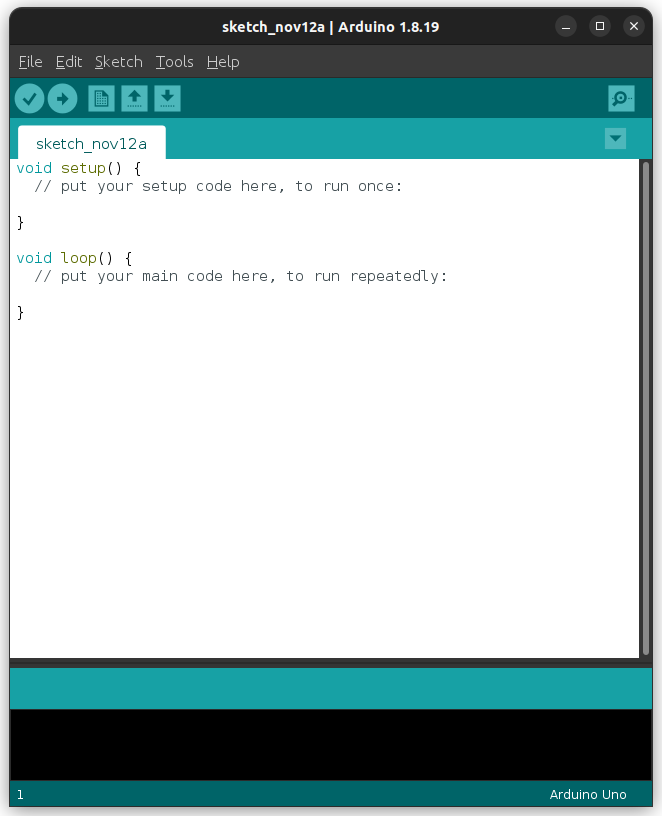
\includegraphics[width=10cm]{arduino-ide-main-window-en}
  \label{fig:arduino-ide-main-window-en}
\end{figure}

\end{document}
